\section{Protocolos Criptográficos Fundamentales en HTTPS}

El funcionamiento de HTTPS descansa sobre un conjunto de protocolos criptográficos que operan de manera coordinada para asegurar las propiedades de confidencialidad, integridad, autenticación y protección contra ataques avanzados. Estos protocolos, definidos principalmente en el marco de la familia \textit{Transport Layer Security} (TLS), constituyen la columna vertebral de las comunicaciones seguras en la web contemporánea y han sido sometidos a exhaustivos análisis formales y evaluaciones empíricas \cite{rfc8446, dowling2015}.

En esta sección se describen los principales protocolos criptográficos que intervienen en HTTPS, abordando su estructura, funcionamiento interno y su relevancia dentro del ecosistema de seguridad digital.

\subsection{Transport Layer Security (TLS)}

TLS es el protocolo criptográfico central de HTTPS y proporciona un canal seguro mediante el cual se transporta HTTP. Su diseño modular permite separar claramente las etapas de negociación, autenticación y protección de datos. La especificación vigente de TLS 1.3, definida en RFC 8446, introduce mejoras sustanciales en seguridad, desempeño y simplicidad arquitectónica respecto a versiones anteriores \cite{rfc8446}.

TLS funciona mediante dos componentes principales:

\begin{enumerate}
    \item \textbf{Handshake TLS}: Encargado de la autenticación de las partes, la negociación de algoritmos criptográficos y el establecimiento de claves de sesión con \textit{Perfect Forward Secrecy}. TLS 1.3 reduce la complejidad del handshake tradicional, elimina algoritmos inseguros y minimiza rondas de comunicación, lo cual incrementa la seguridad y reduce la latencia.
    
    \item \textbf{Record Protocol}: Encargado de encapsular y proteger los datos de aplicación mediante cifrado autenticado (AEAD). Asegura que cada mensaje cuente con integridad, confidencialidad y autenticidad mediante el uso de algoritmos robustos como AES-GCM o ChaCha20-Poly1305 \cite{rfc7525}.
\end{enumerate}

La arquitectura general de TLS ha sido objeto de análisis formales rigurosos que validan sus propiedades criptográficas bajo modelos adversariales de alto nivel \cite{bhargavan2014}.

\subsection{Handshake TLS 1.3}

El \textit{handshake} de TLS 1.3 constituye una de las transformaciones más significativas en la evolución del protocolo. A diferencia de versiones anteriores, TLS 1.3 implementa un proceso simplificado que consta de menos mensajes y elimina mecanismos considerados vulnerables, como RSA para intercambio de claves o el uso de suites sin PFS \cite{krawczyk2016}.

Los objetivos fundamentales del handshake son:

\begin{itemize}
    \item \textbf{Autenticación del servidor} mediante certificados digitales X.509 basados en RSA o ECDSA.
    \item \textbf{Establecimiento de claves efímeras} mediante ECDHE o DHE, lo cual garantiza Perfect Forward Secrecy.
    \item \textbf{Derivación jerárquica de claves} usando HKDF (HMAC-based Key Derivation Function) en conjunto con funciones hash de la familia SHA-2.
    \item \textbf{Validación de integridad y autenticidad} mediante firmas digitales y MACs integrados en los algoritmos AEAD.
\end{itemize}

TLS 1.3 también introduce mecanismos optimizados como:

\begin{itemize}
    \item \textbf{0-RTT (Zero Round Trip Time)} para acelerar la conexión en sesiones previamente establecidas, aunque con advertencias de seguridad debido a la posibilidad de ataques de repetición.
    \item \textbf{Key Update} para rotación continua de claves durante sesiones prolongadas.
\end{itemize}

\begin{figure}[H]
    \centering
    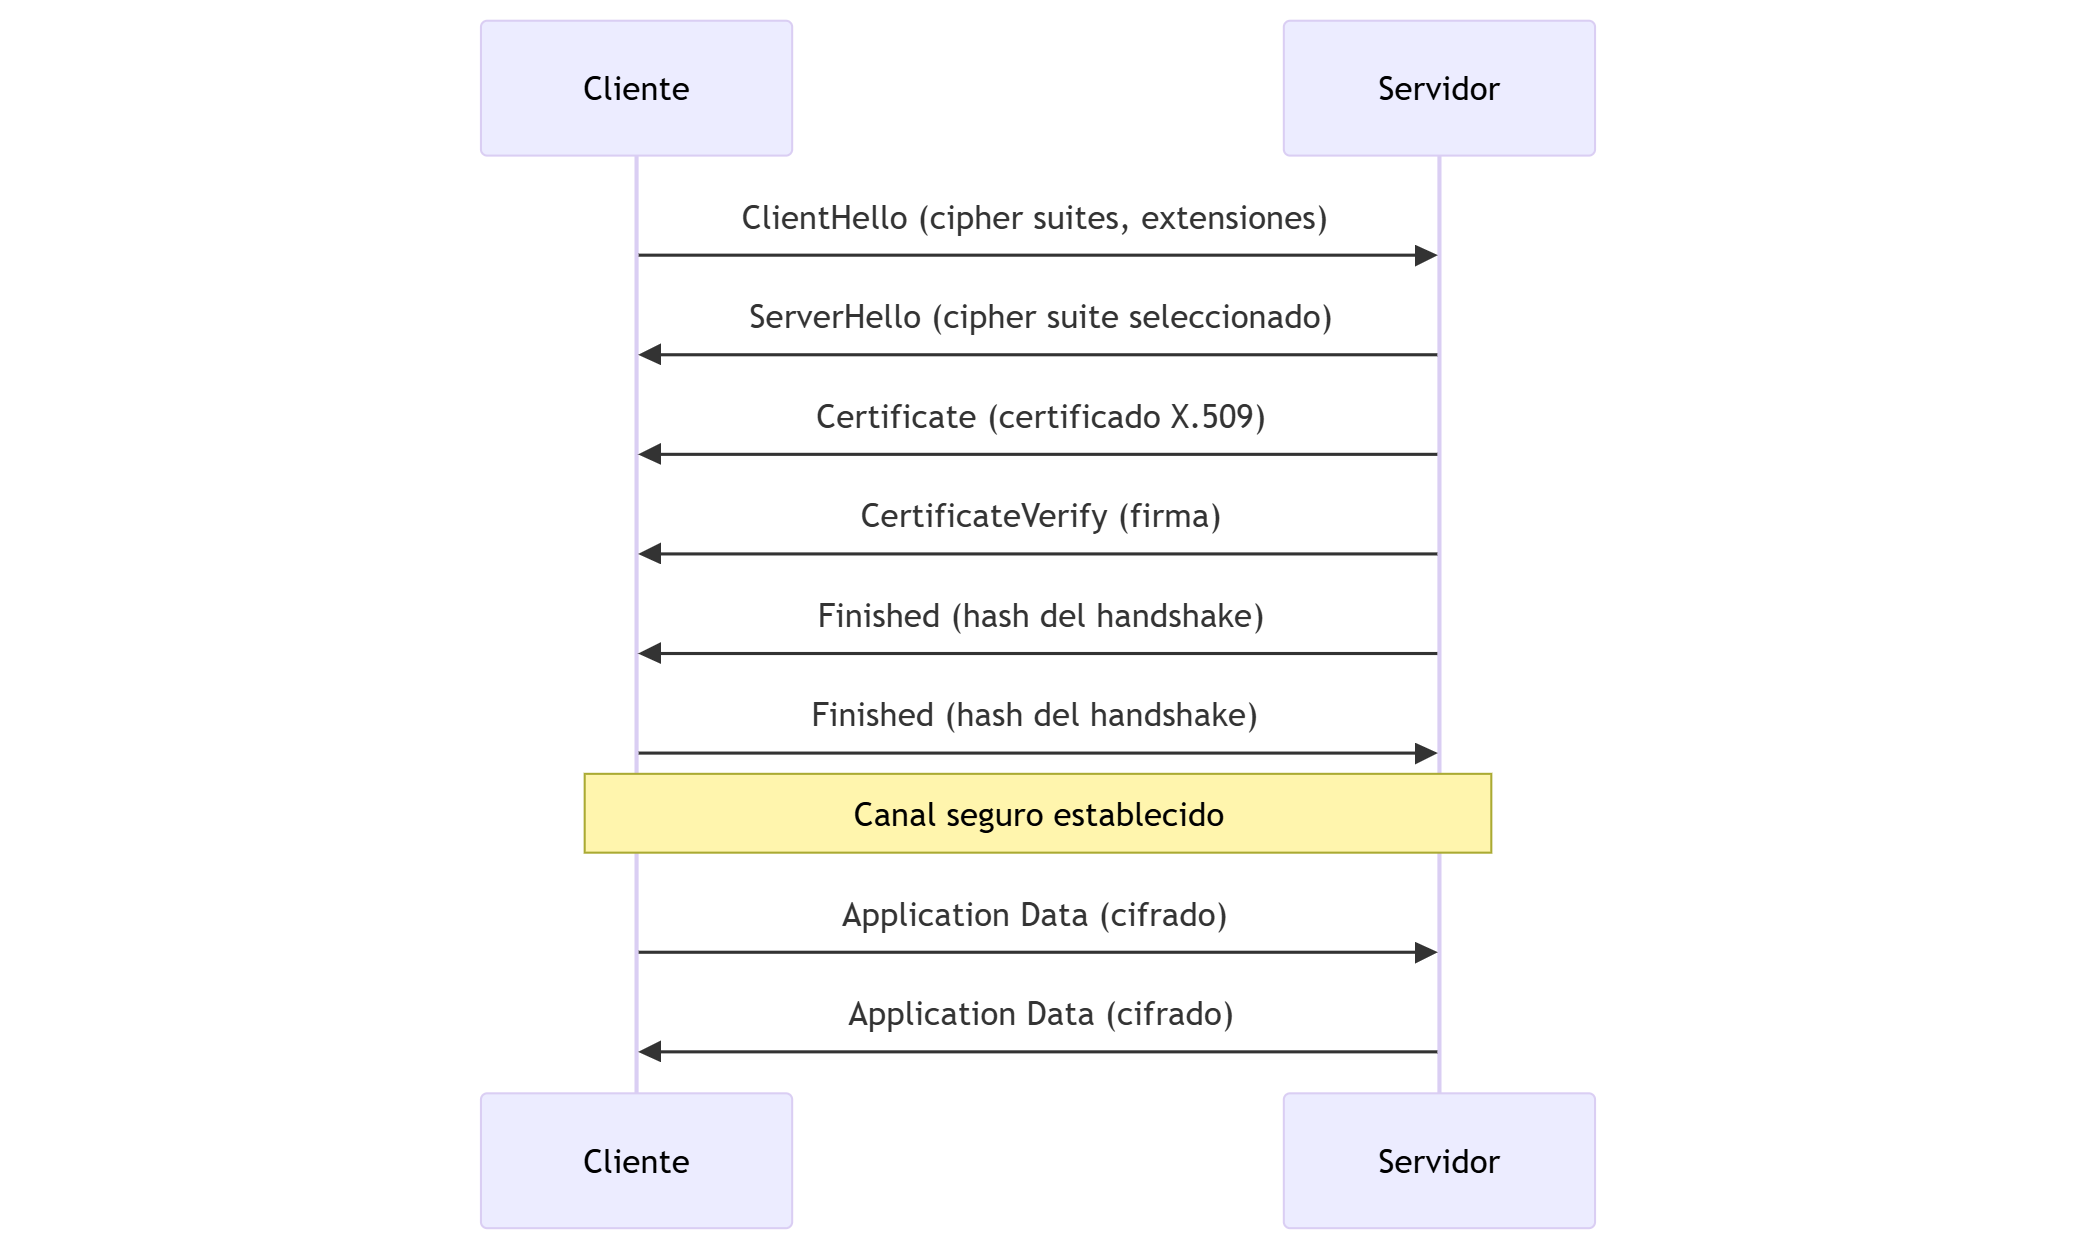
\includegraphics[width=0.95\linewidth]{assets/images/mermaid-diagram-2025-11-29-210558.png}
    \caption{Flujo del Handshake TLS 1.3 en HTTPS}
    \label{fig:tls13-sequence}
\end{figure}


\subsection{X.509 y la Infraestructura de Clave Pública (PKI)}

La autenticación del servidor en HTTPS depende de la infraestructura global de certificados digitales X.509, definida en el estándar RFC 5280 \cite{rfc5280}. La PKI constituye un ecosistema complejo que incluye Autoridades Certificadoras (CA), listas de revocación y mecanismos de validación en tiempo real.

Los componentes fundamentales incluyen:

\begin{itemize}
    \item \textbf{Certificados X.509}: Documentos firmados criptográficamente que vinculan la clave pública del servidor con su identidad.
    \item \textbf{Cadena de confianza}: Secuencia jerárquica que conecta el certificado del servidor con una autoridad raíz confiable.
    \item \textbf{OCSP (Online Certificate Status Protocol)}: Protocolo para verificar en tiempo real si un certificado ha sido revocado.
    \item \textbf{CRL (Certificate Revocation List)}: Listados periódicos de certificados inválidos publicados por las CA.
\end{itemize}

Estudios recientes han revelado limitaciones en la eficacia de los mecanismos de revocación, lo cual motivó mejoras como OCSP Stapling y el impulso hacia certificación de corta duración \cite{liu2015, helme2024}.

\subsection{HTTP Strict Transport Security (HSTS)}

HSTS es un protocolo complementario que refuerza el uso obligatorio de HTTPS en un dominio. Mediante un encabezado especial enviado por el servidor, el navegador instruye a futuras conexiones a utilizar exclusivamente HTTPS, incluso si el usuario intenta acceder mediante HTTP.

Sus objetivos principales son:

\begin{itemize}
    \item Prevenir ataques de \textit{downgrade} hacia HTTP.
    \item Impedir interceptación mediante ataques Man-in-the-Middle en la primera conexión.
    \item Fortalecer la transición inicial hacia HTTPS en sitios previamente no seguros.
\end{itemize}

HSTS ha demostrado reducir significativamente el riesgo asociado a redes inseguras o interceptores pasivos, convirtiéndose en una práctica estándar en la seguridad web moderna.

\subsection{OCSP Stapling}

OCSP Stapling es una mejora del protocolo OCSP tradicional. Permite al servidor adjuntar al handshake una prueba reciente de validez del certificado, firmada por la autoridad emisora. Esta técnica reduce carga sobre las CA, mejora la privacidad del usuario y acelera la validación del certificado.

Debido a fallos documentados en la disponibilidad y confiabilidad de OCSP, el uso de OCSP Stapling se ha convertido en una práctica recomendada para despliegues seguros \cite{liu2015}.

\subsection{DNS over HTTPS (DoH) y Protocolos Asociados}

Aunque no forma parte directa de TLS, DNS over HTTPS (DoH) se ha convertido en un protocolo complementario fundamental para proteger consultas DNS mediante un canal HTTPS seguro. DoH cifra solicitudes DNS, mitigando ataques como espionaje de tráfico, manipulación de resoluciones y filtrado malicioso.

Su estandarización refuerza el ecosistema de privacidad al mover una de las funciones más vulnerables del sistema de nombres hacia un entorno totalmente cifrado.

\subsection{Síntesis General de los Protocolos Criptográficos}

Los protocolos criptográficos que sustentan HTTPS forman un ecosistema interdependiente orientado a garantizar comunicaciones seguras de extremo a extremo. TLS, la infraestructura PKI, mecanismos de validación, y protocolos complementarios como HSTS y OCSP Stapling se integran para proporcionar un modelo robusto frente a adversarios modernos. Su evolución continua permite asegurar compatibilidad, resiliencia operativa y alineación con las mejores prácticas de seguridad digital contemporánea.
